\documentclass[12pt]{report}

\usepackage[top=2cm, bottom=2cm, left=3.5cm, right=2cm, a4paper]{geometry}
\usepackage{titletoc}
\usepackage{tikz}
\usepackage{epigraph}
\usepackage{xpatch}
\usepackage{lmodern}
\usepackage[utf8]{vietnam}
\usepackage{ragged2e}
\usepackage{fancyhdr}
\usepackage[hidelinks]{hyperref}
\usepackage{float}
\usepackage{array}
\usepackage{amssymb}
\newcolumntype{C}{>{\centering\arraybackslash}m{3cm}}

%source codes
\definecolor{bluekeywords}{rgb}{0.13,0.13,1}
\definecolor{greencomments}{rgb}{0,0.5,0}
\definecolor{redstrings}{rgb}{0.9,0,0}

\usepackage{listings}
\lstset{language=[Sharp]C,
showspaces=false,
showtabs=false,
breaklines=true,
showstringspaces=false,
breakatwhitespace=true,
escapeinside={(*@}{@*)},
commentstyle=\color{greencomments},
keywordstyle=\color{bluekeywords}\bfseries,
stringstyle=\color{redstrings},
basicstyle=\ttfamily
    backgroundcolor=\color{background},
}
\usepackage{xcolor}

\colorlet{punct}{red!60!black}
\definecolor{background}{HTML}{EEEEEE}
\definecolor{delim}{RGB}{20,105,176}
\colorlet{numb}{magenta!60!black}
\lstdefinelanguage{json}{
    basicstyle=\normalfont\ttfamily,
    numbers=left,
    numberstyle=\scriptsize,
    stepnumber=1,
    numbersep=8pt,
    showstringspaces=false,
    breaklines=true,
    frame=lines,
    backgroundcolor=\color{background},
    literate=
     *{0}{{{\color{numb}0}}}{1}
      {1}{{{\color{numb}1}}}{1}
      {2}{{{\color{numb}2}}}{1}
      {3}{{{\color{numb}3}}}{1}
      {4}{{{\color{numb}4}}}{1}
      {5}{{{\color{numb}5}}}{1}
      {6}{{{\color{numb}6}}}{1}
      {7}{{{\color{numb}7}}}{1}
      {8}{{{\color{numb}8}}}{1}
      {9}{{{\color{numb}9}}}{1}
      {:}{{{\color{punct}{:}}}}{1}
      {,}{{{\color{punct}{,}}}}{1}
      {\{}{{{\color{delim}{\{}}}}{1}
      {\}}{{{\color{delim}{\}}}}}{1}
      {[}{{{\color{delim}{[}}}}{1}
      {]}{{{\color{delim}{]}}}}{1},
}

\renewcommand{\lstlistingname}{Mã nguồn}
\renewcommand{\lstlistlistingname}{Danh sách mã nguồn}

% Part ToC
\usepackage{titlesec,titletoc}  

\titleclass{\part}{top}
\titleformat{\part}
[display]
{\centering\normalfont\Huge\bfseries}
{\titlerule[2pt]\vspace{15pt}\MakeUppercase{\partname} \thepart}
{0pt}
{\vspace{1pc}\LARGE}[{\vspace{1pc}\titlerule[1pt]}]

\setcounter{secnumdepth}{5}


%Vietnamese
\usepackage[utf8]{inputenc}

%Line spacing
\renewcommand{\baselinestretch}{1.2}
\usepackage{tikz}
\usetikzlibrary{calc}
\newcommand\HRule{\rule{\textwidth}{1pt}}

%Page style
\pagestyle{fancy}
\fancyhf{}
\rhead{}
\lhead{}
\lfoot{\textit{Sinh viên thực hiện: Trần Hoài Nam, 20122123, CNTT2 04 K57}}
\rfoot{\thepage}
\renewcommand{\footrulewidth}{1pt}

% Redefine the plain page style
% \fancypagestyle{plain}{%
%   \fancyhf{}%
%   \lfoot{\textit{Sinh viên thực hiện: Trần Hoài Nam, 20122123, CNTT2 04 K57}}
%   \rfoot{\thepage}
%   \renewcommand{\headrulewidth}{0pt}% Line at the header invisible
%   \renewcommand{\footrulewidth}{1pt}% Line at the footer visible
% }

%ToC page style
\usepackage{tocloft}

\renewcommand\cftsecleader{\cftdotfill{\cftdotsep}}
\renewcommand\cftchapleader{\cftdotfill{\cftdotsep}}
\renewcommand\cftpartleader{\cftdotfill{\cftnodots}}

% Quote box
\usepackage{framed}
\usepackage[strict]{changepage}    

%Defining colour with different models.
\definecolor{lightgray}{gray}{0.95}
\definecolor{mygray}{gray}{0.8} 

\newenvironment{formal}{%
  \def\FrameCommand{%
    \hspace{1pt}%
    {\color{mygray}\vrule width 6pt}%
    {\color{lightgray}\vrule width 4pt}%
    \colorbox{lightgray}%
  }%
  \MakeFramed{\advance\hsize-\width\FrameRestore}%
  \noindent\hspace{-4.55pt}% disable indenting first paragraph
  \begin{adjustwidth}{}{7pt}%
  \vspace{2pt}\vspace{2pt}%
}
{%
  \vspace{2pt}\end{adjustwidth}\endMakeFramed%
}

%Replaceable project name
\newcommand{\project}{VVC}

\begin{document}

\begin{titlepage}

	\begin{tikzpicture}[remember picture, overlay]
	  \draw[line width = 1pt] ($(current page.north west) + (3.5cm,-2cm)$) rectangle ($(current page.south east) + (-2cm,2cm)$);
	\end{tikzpicture}

	\begin{center}
		\vspace{0.3cm}
		\begin{large}
		TRƯỜNG ĐẠI HỌC BÁCH KHOA HÀ NỘI	\\
		VIỆN CÔNG NGHỆ THÔNG TIN VÀ TRUYỀN THÔNG	\\
		\_\_\_\_\_\_\_\_*\_\_\_\_\_\_\_\_ \\[4.5cm]
		\end{large}
			
		{\huge ĐỒ ÁN }\\	
		{\Huge \textbf{TỐT NGHIỆP ĐẠI HỌC}}\\[0.3cm]
		{\Large NGÀNH CÔNG NGHỆ THÔNG TIN}  \\[4cm]
	
		{\Large \textbf{ĐỀ TÀI}}\\[0.3cm]		
		{\large XÂY DỰNG CHATBOT ĐIỀU KHIỂN ĐIỆN THOẠI BẰNG TIẾNG VIỆT} \\[2.5cm]
	\end{center}
	
	\begin{justify}

		\hspace{6cm} Sinh viên thực hiện \hspace{0.2cm}: \textbf{Trần Hoài Nam} \hspace{0.3cm}

		\noindent \hspace{6cm} Lớp \hspace{3.0cm}: CNTT-TT2 04, K57 \hspace{0.3cm}

		\noindent \hspace{6cm} Giáo viên hướng dẫn\hspace{0.14cm} : ThS. \textbf{Trịnh Thành Trung} \hspace{0.3cm} \\[2.5cm]
		
	\end{justify}

	\begin{center}
		Hà Nội, 5/2017
	\end{center}
	
\end{titlepage}

\pagenumbering{roman}
\setcounter{page}{1}

% Phiếu giao nhiệm vụ đồ án tốt nghiệp
\begin{center}
{\large \textbf{PHIẾU GIAO NHIỆM VỤ ĐỒ ÁN TỐT NGHIỆP}}
\end{center}

\noindent 1. Thông tin về sinh viên
\begin{itemize}
	\item Họ và tên: Trần Hoài Nam.
	\item MSSV: 20122123.
	\item Lớp: CNTT-TT2 04 K57.
\end{itemize}

\noindent 2. Mục đích nội dung của ĐATN\\
\noindent Đề xuất ứng dụng chatbot bằng giọng nói Tiếng Việt trong điều khiển nhà thông minh.\\[0.4cm]
\noindent 3. Các nhiệm vụ cụ thể của ĐATN
\begin{itemize}
	\item Xây dựng chatbot hiểu được yêu cầu từ người dùng bằng Tiếng Việt
	\item Hỗ trợ giao tiếp bằng giọng nói
	\item Cải thiện khả năng phân tích giọng nói thành văn bản
\end{itemize}

\noindent 4. Lời cam đoan của sinh viên:\\
Tôi - \textit{Trần Hoài Nam} - cam kết ĐATN là công trình nghiên cứu của bản thân tôi dưới sự hướng dẫn của \textit{ThS. Trịnh Thành Trung}.

\noindent Các kết quả nêu trong ĐATN là trung thực, không phải là sao chép hoàn văn của bất kỳ công trình nào khác.\\[0.5cm]
  
\begin{minipage}{0.3\textwidth}
\hspace{1cm}
\end{minipage}
~
\begin{minipage}{0.6\textwidth}
\centering
\textit{Hà Nội, ngày \hspace{0.3cm} tháng  \hspace{0.3cm} năm 2017.} \\
Tác giả ĐATN \\[2cm]
\textit{Trần Hoài Nam}
\end{minipage}\\[0.5cm]
\noindent 5. Xác nhận của giáo viên hướng dẫn về mức độ hoàn thành của ĐATN và cho phép bảo vệ:
  
\begin{minipage}{0.3\textwidth}
\hspace{1cm}
\end{minipage}
~
\begin{minipage}{0.6\textwidth}
\centering
\textit{Hà Nội, ngày \hspace{0.3cm} tháng  \hspace{0.3cm} năm 2017.} \\
Giáo viên hướng dẫn\\[2cm]
\textit{ThS. Trịnh Thành Trung}
\end{minipage}\\[0.5cm]

\newpage

% lỜI CẢM ƠN
\begin{center}
{\large \textbf{LỜI CẢM ƠN}}
\end{center}
Để hoàn thành đồ án tốt nghiệp này, em xin chân thành cảm ơn các thầy cô giáo tại Viện Công nghệ thông tin và Truyền thông, Trường Đại học Bách Khoa Hà Nội đã tận tình chỉ dạy cho em từ những ngày đầu tiên được tiếp xúc với Công nghệ thông tin và lập trình. Những kiến thức qua các môn học từ cơ bản đến nâng cao mà các thầy cô truyền đạt đã giúp em có thể xây dựng cho mình một nền tảng vững chắc để có thể tiếp tục nghiên cứu và phát triển, mở rộng đến những kiến thức mới theo định hướng bản thân.

Đặc biệt, em xin chân thành cảm ơn thầy ThS. Trịnh Thành Trung, người đã định hướng đề tài và hướng dẫn em tận tình từ những ngày đầu làm đồ án, giải đáp những thắc mắc cũng như gỡ rối cho em những lúc khó khăn nhất để em có thể hoàn thành tốt đồ án tốt nghiệp này.

Tôi cũng xin chân thành cảm ơn những anh chị đồng nghiệp tại công ty TNHH Niteco đã giúp đỡ, chỉ bảo tận tình để tôi có được những kiến thức quý báu và cái nhìn tổng quan về lập trình nói chung, điều đó đã giúp tôi rất nhiều trong quá trình hoàn thành đồ án tốt nghiệp.

Cuối cùng, tôi xin gửi lời cảm ơn tới gia đình của tôi, và những người bạn bè thân thiết nhất, đã luôn ủng hộ và động viên trong những lúc khó khăn để tôi có thể hoàn thành đồ án tốt nghiệp này.

\newpage

% TÓM TẮT
\begin{center}
{\large \textbf{TÓM TẮT NỘI DUNG ĐỒ ÁN TỐT NGHIỆP}}
\end{center}
\addcontentsline{toc}{chapter}{Tóm tắt nội dung đồ án tốt nghiệp}

\noindent Họ và tên sinh viên: Trần Hoài Nam \\
Lớp: CNTT-TT2 04 K57\\
Tên đề tài: \\
Giáo viên hướng dẫn: ThS. Trịnh Thành Trung.\\
\begin{itemize}
	\item Yêu cầu đồ án:
		\begin{itemize}
			\item Nghiên cứu xây dựng ứng dụng chatbot hỗ trợ điều khiển nhà thông minh bằng giọng nói Tiếng Việt
			\item Cải thiện kết quả phân tích giọng nói thành văn bản
			\item Xây dựng chatbot có thể phân tích yêu cầu từ phía người dùng
		\end{itemize}
	\item Kết quả đạt được:
		\begin{itemize}
			\item Xây dựng thành công thư viện chatbot phân tích yêu cầu từ phía người dùng và trả lời
			\item Tích hợp thư viện chatbot vào ứng dụng điều khiển điện thoại bằng giọng nói
			\item Cải thiện độ chính xác của nhận diện giọng nói sử dụng mô hình ngôn ngữ
		\end{itemize}
	\item Công cụ sử dụng:
		\begin{itemize}
			
			\item SRILM - công cụ hỗ trợ tính toán mô hình ngôn ngữ
			\item Wit.ai - công cụ 
		\end{itemize}
	\item Đánh giá:
	\item Ý nghĩa đồ án:
\end{itemize}

\newpage

% ABSTRACT
\begin{center}
{\large \textbf{ABSTRACT OF THESIS}}
\end{center}
\addcontentsline{toc}{chapter}{Abstract of Thesis}

\noindent Full name: Trần Hoài Nam \\
Class: CNTT-TT2 04 K57\\
Title of Thesis: \\
Supervisor: ThS. Trịnh Thành Trung.\\
\begin{itemize}
	\item Requirements:
	\item Achievements:
	\item Tools:
	\item Evaluations:
	\item Meaning of Thesis:
\end{itemize}

\newpage

\tableofcontents
\newpage

\listoffigures
\addcontentsline{toc}{chapter}{Danh sách hình vẽ}
\newpage

\listoftables
\addcontentsline{toc}{chapter}{Danh sách bảng}

\newpage
\lstlistoflistings
\addcontentsline{toc}{chapter}{Danh sách mã nguồn}

% FOREWORD
\newpage
\begin{center}
{\large \textbf{LỜI NÓI ĐẦU}}
\end{center}
\addcontentsline{toc}{chapter}{Lời nói đầu}
Tại thời điểm hiện tại, công nghệ thông tin đang phát triển và hiện hữu trong đời sống của mỗi người, cùng với đó là sự tiến bộ vượt bậc trong lĩnh vực trí tuệ nhân tạo, giúp tạo ra những sản phẩm công nghệ có khả năng xử lý gần như con người tại một khía cạnh cụ thể, để thay thế và giải quyết một phần nhu cầu từ phía người sử dụng. Điện thoại thông minh (smart phone) ra đời đã và đang là sản phẩm công nghệ không thể thiếu với mỗi người trong cuộc sống hiện đại. Tuy nhiên một điểm bất lợi cố hữu của điện thoại thông minh là việc nhập nội dung bằng tay chậm do bàn phím ảo nhỏ, cũng như muốn thực hiện các chức năng cần thao tác nhiều, nhìn vào màn hình, gây ra những khó khăn trong việc sử dụng, đặc biệt là đối với những người lái xe hơi cần sự tập trung mà vẫn muốn sử dụng điện thoại thông minh để giải quyết công việc.

Trên thế giới hiện nay, những ông lớn như Google hay Apple đã cho ra đời rất nhiều sản phẩm liên quan đến các trợ lý ảo để ra lệnh bằng giọng nói và điều khiển điện thoại như Google Now (Google Assistant) hay Siri của Apple. Những phần mềm này đều được tích hợp trong các hệ điều hành của các điện thoại thông minh thế hệ mới, tuy nhiên vẫn đang chỉ hỗ trợ Tiếng Anh và chưa hiểu được yêu cầu bằng Tiếng Việt. Vì vậy, trong đồ án tốt nghiệp này, em xin đề xuất giải pháp cho vấn đề xây dựng chatbot điều khiển điện thoại thông minh bằng giọng nói Tiếng Việt.

Đồ án tốt nghiệp được chia thành 2 phần chính. Phẩn một là đặt vấn đề của đồ án và định hướng giải pháp cho vấn đề và phần hai sẽ là những kết quả nghiên cứu đã đạt được trong quá trình giải quyết vấn đề của đồ án.

\newpage
\setcounter{page}{1}
\pagenumbering{arabic}

\newcommand{\alice}{A.L.I.C.E }

\part{Đặt vấn đề và định hướng giải pháp}

\startcontents[parts]
\printcontents[parts]{}{-1}{\setcounter{tocdepth}{1}}

\chapter{Đặt vấn đề}
\section{Tổng quan về chatbot và các hệ thống trợ lí ảo}
\subsection{Chatbot}
Theo Wikipedia định nghĩa, ``một \textit{chatbot} (hay có thể gọi là talkbot, chatterbot hay chatterbox ...) là một chương trình máy tính mà tạo ra những cuộc hội thoại thông qua các phương thức nghe và nhập văn bản''. Một chatbot thường được thiết kế và phát triển để có thể ứng xử và cảm giác như một người thật trong những tình huống cụ thể như tin nhắn trả lời tự động hay hệ thống cung cấp thông tin cần thiết cho người dùng. Những công việc này sẽ luôn cần một hoặc nhiều người trực tổng đài để có thể phục vụ, giải đáp các thắc mắc từ phía người dùng nếu như không có các hệ thống chatbot trả lời tự động. Hay đơn giản là khi một người muốn giải trí và cần một ai đó để trò chuyện, không những thế người đó còn cần phải hiểu mình, những hệ thống chatbot có thể giúp giải quyết những vấn đề như vậy.

Từ những năm 50 của thế kỉ trước, chatbot đã được nhen nhóm và có những bước đi đầu tiên. Vào năm 1950, \textit{Alan Turing} đã xuất bản quyển sách \textit{Computing Machinery and Intelligence} mà sau này được gọi là ``bài kiểm tra Turing'' và được coi như là một tiêu chuẩn để do sự thông minh của một chương trình máy tính. Tiêu chuẩn này phụ thuộc vào khả năng của chương trình máy tính đó khi đóng giả là một con người và tham gia vào một cuộc hội thoại thời gian thực sao cho đủ tốt để những giám khảo không thể phân biệt được đây là cuộc trò chuyện giữa người và máy tính. Bài kiểm tra Turing đã được ứng dụng rõ ràng ở trong \textit{ELIZA} - một chương trình của Joseph Weizenbaum được phát hành năm 1966. Ứng dụng có khả năng đánh lừa người dùng và làm cho họ không thể phân biệt được là đang nói chuyện với máy tính chứ không phải con người thật.

Phương pháp chính trong việc thực hiện của ELIZA là nhận diện câu hoặc một phần của câu nói từ phía đầu vào và đầu ra là một câu trả lời được chọn tương ứng với đầu vào từ một tập dữ liệu đã chuẩn bị trước trong hệ thống. Tập dữ liệu này được chuẩn bị bởi chính con người thật nên các cặp \textit{Câu hỏi - Câu trả lời} đều khá phù hợp và tạo ra một cuộc hội thoại có ý nghĩa, khiến người dùng thật sự bất ngờ về khả năng có thể hiểu câu hỏi và đưa ra câu trả lời phù hợp của chatbot.

Trong quá trình phát triển, ngoài ELIZA còn có rất nhiều những chatbot khác được hình thành, có thể kể đến như PARRY (1972), \alice (1995) hay Jabberwacky (1997) ... Những chatbot này đều có chung một cách vận hành chính là \textit{pattern matching} (phù hợp mẫu), tức là chọn ra những câu trả lời phù hợp từ tập những mẫu câu đã có sẵn trong hệ thống được xây dựng bởi chính người thật. Chatbot \alice sử dụng \textit{AIML} (Artificial Intelligence Markup Language - Ngôn ngữ trí tuệ nhân tạo đánh dấu) là một ngôn ngữ có dạng XML, sử dụng các thẻ để quy định các cặp câu hỏi - câu trả lời, kèm theo một số điều kiện hay các lựa chọn khác, để hệ thống dựa vào đó và đưa ra các câu trả lời phù hợp trong cuộc hội thoại.

\begin{figure}[H]
  \centering
    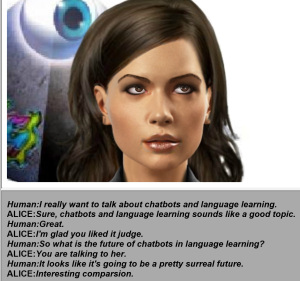
\includegraphics[width=10cm]{Pics/Chap1/alice.jpg}
  \caption{Một cuộc hội thoại giữa người thật và \alice}
\end{figure}

Ta có thể thấy những câu trả lời của \alice tương đối phù hợp trong ngữ cảnh của cuộc hội thoại, không khác nhiều so với cách trả lời của người thật, tạo cảm giác như chatbot có thể hiểu được câu hỏi và trả lời một cách phù hợp. Tuy nhiên trong nhiều lĩnh vực ngày nay, chatbot không chỉ cần trong việc hỗ trợ tìm kiếm hay cung cấp thông tin cho người dùng, mà còn cần dùng cho những việc hoàn toàn tự động và có thể hiểu câu hỏi từ phía người dùng như đặt chỗ chuyến bay, đồ ăn ... hay điều khiển các thiết bị. Điều này dẫn đến một phương pháp khác trong việc xây dựng chatbot thực sự có trí thông minh, trí tuệ nhân tạo, đó là sử dụng \textit{Xử lý ngôn ngữ tự nhiên} (NLP - natural language processing) nhằm phân tích được cú pháp, ý nghĩa câu nói của người dùng đang hướng tới, hiểu rõ yêu cầu từ phía người dùng, để từ đó có thể đáp ứng những yêu cầu đó.

\subsection{Hệ thống trợ lý ảo}
Một \textit{trợ lý ảo} là một hệ thống phần mềm giúp thực hiện các nhiệm vụ hay các dịch vụ cho mỗi một cá nhân. Mỗi trợ lý ảo sẽ giúp cho người sử dụng thực hiện một nhiệm vụ trên một môi trường cụ thể như máy tính hay thiết bị điện thoại thông minh, hoặc trong chính căn nhà của mình để điều khiển các thiết bị nội thất trong ngôi nhà. Có nhiều phương thức để một trợ lý ảo có thể tương tác với người dùng như:

\begin{itemize}
	\item Văn bản (text)
	\item Âm thanh (voice)
	\item Ảnh được tải lên
\end{itemize}

Chatbot chính là một trợ lý ảo sử dụng văn bản hoặc giọng nói để cung cấp cho người dùng thông tin cần thiết hay chỉ đơn giản là trò chuyện với người dùng. Bên cạnh đó còn các trợ lý ảo được xây dựng để giúp người dùng thực hiện một nhiệm vụ nào đó như Google Assistant thông qua Google Allo có thể giúp người dùng tìm kiếm thông tin hay đặt lịch, giải trí và các nhiệm vụ cá nhân khác, hoặc thông qua Google Home để điều khiển các thiết bị thông minh trong ngôi nhà. Tại thời điểm hiện tại, các ông lớn trong ngành công nghệ như Google, Apple, Amazon hay Microsoft đã cho ra đời những trợ lý ảo của riêng mình và vẫn tiếp tục hoàn thiện để những trợ lý này trở thành một phần không thể thiếu trong cuộc sống hiện đại. Trong một bài viết trên trang Business Insider{\footnote{http://www.businessinsider.com/siri-vs-google-assistant-cortana-alexa-2016-11}} vào tháng 11/2016 đã đề cập đến một cuộc thi nhỏ giữa các trợ lý ảo của các ông lớn kể trên là Siri của Apple, Alexa của Amazon, Cortana của Microsoft và Google Assistant của Google. Kết quả được đánh giá dựa trên nhiều tiêu chí, mỗi trợ lý ảo đều có một điểm mạnh hay điểm yếu riêng trong những mục mà mình chưa hỗ trợ, tuy nhiên đánh giá chung là những trợ lý ảo này đều rất thông minh và có thể hiểu tối đa yêu cầu từ phía người dùng. 

\begin{figure}[H]
  \centering
    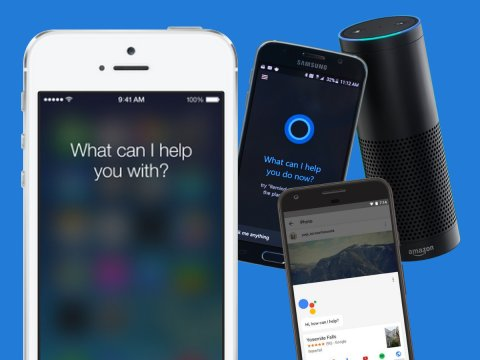
\includegraphics[width=10cm]{Pics/Chap1/virtual-assistants.png}
  \caption{Hình ảnh nền tảng của những trợ lý ảo nổi tiếng}
\end{figure}

Những trợ lý ảo đang ngày càng phát triển cả về trí thông minh lẫn những lĩnh vực hiện hữu trong cuộc sống. Tuy nhiên những trợ lý ảo này mới chỉ phát triển trên ngôn ngữ là Tiếng Anh và hoàn toàn không có khả năng hiểu Tiếng Việt, gây ra cản trở trong mong muốn được tiếp cận những công nghệ tiên tiến trên thế giới của người Việt. Những trợ lý ảo đó có thể hiểu và phân tích được yêu cầu của người dùng bằng Tiếng Việt đã là một khó khăn, và sẽ khó khăn hơn nếu như người dùng sử dụng giọng nói để đưa yêu cầu vào hệ thống. Nhưng với sự hỗ trợ của những công ty lớn như Google trong việc nhận diện giọng nói Tiếng Việt và các nền tảng xây dựng chatbot sử dụng NLP, vấn đề này sẽ không còn bất khả thi nữa. Trong đề tài nghiên cứu này sẽ nêu rõ giải pháp để giải quyết vấn đề xây dựng chatbot để điều khiển điện thoại bằng giọng nói Tiếng Việt, và xa hơn nữa sẽ hỗ trợ để điều khiển các thiết bị trong ngôi nhà thông minh - Smart Home.

\section{Mục đích của đề tài}

Sự tiện dụng và những lợi ích mà chatbot hay những trợ lý ảo mang lại cho con người là vô cùng lớn, giúp cải thiện chất lượng cuộc sống của mọi người trong thời kì công nghệ đang ngày càng phát triển và trở thành một phần không thể thiếu trong đời sống. Ở Việt Nam hiện nay, những công nghệ thông minh cũng đang rất được quan tâm như điện thoại thông minh hay nhà thông minh. Bài viết vào đầu năm 2017{\footnote{http://baoquocte.vn/10-xu-huong-tieu-dung-cong-nghe-nam-2017-42757.html}} của \textit{baoquocte.vn} đã cho biết ``Trí tuệ nhân tạo (AI - Artificial Intelligence) sẽ là xu hướng nổi bật của năm 2017''. Trong bài viết đã nêu rõ sự có mặt khắp mọi nơi của trí tuệ nhân tạo, và có đến 35\% những người sử dụng Internet đều mong muốn có một cố vấn robot có trí tuệ nhân tạo để phục vụ những nhu cầu và lợi ích cá nhân. Bên cạnh đó, thời điểm này cũng đang là thời kì nở rộ của \textit{Internet of Things} - Vạn vật kết nối, khi mà các thiết bị điện tử dù lớn hay nhỏ trong gia đình hay trên các con phố cũng đều có thể kết nối với nhau trong một mạng Internet thống nhất và đều được kiểm soát chỉ thông qua một màn hình nhỏ của thiết bị thông minh như điện thoại hay máy tính bảng. Từ đó nhu cầu để điều khiển các thiết bị này không còn chỉ gói gọn ở trong việc sử dụng các thiết bị thông minh mà còn qua các phương thức khác nhau giọng nói, cử chỉ của tay chân hay thậm chí là sử dụng chính những suy nghĩ trong não bộ của con người.

Số lượng người sử dụng điện thoại thông minh ở Việt Nam cũng là rất cao, lên đến trên 25 triệu người trên tổng số trên 90 triệu dân và con số này sẽ còn tăng mạnh trong năm 2017 và những năm tiếp theo{\footnote{https://news.appota.com/bao-cao-thi-truong-mobile-viet-nam-q3-2016/}}. Cũng trong thời điểm này, có đến 39,8 triệu người Việt Nam sử dụng mạng Internet và khoảng 21,6 triệu người sử dụng Internet thông qua các thiết bị di động, điện thoại thông minh. Có thể thấy xu hướng sử dụng công nghệ ngày càng cao tại Việt Nam, và việc phát triển các sản phẩm trên các thiết bị này là một nhu cầu thiết yếu, đem lại nhiều lợi ích cho các doanh nghiệp Việt Nam nói riêng và nền kinh tế Việt Nam nói chung.

\begin{figure}[H]
  \centering
    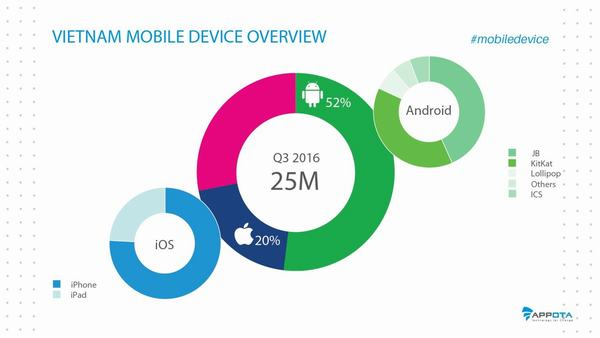
\includegraphics[width=15cm]{Pics/Chap1/mobile-vietnam.jpg}
  \caption{Tổng kết số lượng người sử dụng smart phone ở Việt Nam cuối năm 2016}
\end{figure}

Với những người đang điều khiển các phương tiện giao thông như xe hơi thì việc sử dụng điện thoại thông minh và phải nhìn vào màn hình là một việc nguy hiểm, gây cản trở trong quá trình điều khiển xe, có thể gây ra tai nạn, hay khi sử dụng điện thoại mà người dùng phải thực hiện thao tác tay quá nhiều mới có thể hoàn thành được một nhiệm vụ hay yêu cầu sẽ gây ra cảm giác khó chịu, đặc biệt là việc nhập văn bản bằng tay trên các thiết bị di động thông minh rất khó khăn do bàn phím trên các thiết bị nhỏ, dễ gây nhầm lẫn khi nhập đoạn dài. Vì vậy trong đồ án nghiên cứu này sẽ đề xuất giải pháp để giải quyết cho vấn đề ``\textbf{Xây dựng chatbot điều khiển điện thoại bằng giọng nói Tiếng Việt}''. Đồ án sẽ tập trung vào việc xử lý giọng nói từ phía người dùng và chuyển thành dạng văn bản để có thể phân tích yêu cầu, từ đó xây dựng những tính năng giúp người dùng có thể điều khiển được chiếc điện thoại thông minh bằng chính giọng nói của mình với ngôn ngữ Tiếng Việt.


\chapter{Định hướng giải pháp}

Với vấn đề đã được đặt ra ở phần trên, đồ án đề xuất giải pháp với 2 mục tiêu chính là nhận diện giọng nói Tiếng Việt từ phía người dùng và xây dựng chatbot để phân tích yêu cầu từ phía người dùng (sử dụng \textit{Xử lý ngôn ngữ tự nhiên}).

\section{Nhận diện giọng nói}
\subsection{Khái niệm}
Nhận dạng giọng nói (Nhận dạng tiếng nói) là một quá trình \textit{nhận dạng mẫu}, với mục đích là phân lớp những thông tin đầu vào bằng giọng nói từ phía người dùng thành một chuỗi các kí tự (các từ) đã được học từ trước và lưu trữ lại trong bộ nhớ. Các mẫu là các đơn vị nhận dạng, có thể là một đoạn âm thanh của một từ hay một âm tiết. Nếu như việc nhận dạng chỉ dừng lại ở mức so sánh những mẫu có trong tập học với đoạn âm thanh và chọn ra mẫu trùng khớp nhất thì không có nhiều khó khăn. Những khó khăn cơ bản của nhận diện giọng nói có thể kể đến như:

\begin{itemize}
	\item Cùng là một từ hay một âm tiết cố định nhưng có vô vàn giọng nói khác nhau có thể diễn đạt lại được. Sự khác nhau đó là do âm lượng, tốc độ nói hay môi trường âm học của mỗi người là khác nhau, vì vậy khi chỉ sử dụng một giọng nói để làm mẫu nhận diện thì xác suất để nhận diện đúng và chính xác sẽ rất thấp, không mang lại nhiều giá trị nghiên cứu
	\item Thông thường người dùng sẽ không chỉ nói những câu nói bao gồm một từ đơn lẻ mà là một câu dài mang đủ ý nghĩa, kết hợp từ các từ đơn, từ ghép khác nhau. Việc phân tách được câu nói đó thành những chuỗi những cụm từ liên tục cũng là một việc làm khó khăn
	\item Tạp âm cũng là một phần gây nhiễu và khó khăn lớn trong việc nhận dạng giọng nói. Xác định những thông tin biến thiên nào là tiếng nói có ích và những thông tin nào là tiếng nói không có ích trong việc phân tích cũng là một yếu tố vô cùng quan trọng
\end{itemize}

\noindent Các nghiên cứu về nhận dạng tiếng nói dựa trên ba nguyên tắc cơ bản sau:
\begin{itemize}
	\item Tín hiệu tiếng nói được biểu diễn chính xác bởi các giá trị phổ trong một khoảng thời gian ngắn, nhờ vậy ta có thể trích ra các đặc điểm tiếng nói từ những khoảng thời gian ngắn và dùng các đặc điểm này để nhận dạng tiếng nói
	\item Nội dung của tiếng nói được biểu diễn dưới dạng chữ viết, là một dãy các ký hiệu ngữ âm, vì vậy ý nghĩa của một phát âm được bảo toàn khi chúng ta phiên âm phát âm thành các ký hiệu ngữ âm
	\item Nhận dạng tiếng nói là một quá trình nhận thức. Thông tin về ngữ nghĩa và suy đoán có giá trị trong quá trình nhận dạng tiếng nói, nhất là khi thông tin về âm học{\footnote{Âm học là một nhánh của vật lý học, nghiên cứu về sự lan truyền của sóng âm thanh trong các loại môi trường và sự tác động qua lại của nó với vật chất}} là không rõ ràng
\end{itemize}

Nhận diện giọng nói là một việc làm rất khó khăn từ việc xây dựng được bộ dữ liệu mẫu để so sánh đến việc xây dựng các mô hình thống kê xác suất để tổng quát hóa từ những mẫu tiếng nói thành những biến thiên quan trọng trong việc nhận dạng. Một số cách tiếp cận nhận dạng tiếng nói bằng thống kê bao gồm: mô hình Markov ẩn, mạng nơ-ron, sử dụng cơ sở tri thức \ldots.

\subsection{Google Speech Recognition API}
% .3cm
\subsubsection{Công cụ hỗ trợ nhận diện giọng nói}
Có rất nhiều các thư viện giúp nhận dạng giọng nói trên rất nhiều nền tảng, ngôn ngữ lập trình khác nhau và các ngôn ngữ của các quốc gia khác nhau, tuy nhiên với Tiếng Việt thì dường như không có nhiều vì để có thể nhận diện được thì cần một bộ dữ liệu mẫu vô cùng lớn mới có thể tăng độ chính xác lên được, và việc làm này gặp rất nhiều khó khăn ở Việt Nam do nguồn cung cấp giọng nói mẫu đầu vào không có. Cũng đã có những nhóm nghiên cứu nhận diện giọng nói Tiếng Việt ở Việt Nam, tuy nhiên chỉ dừng lại ở mức nhận diện một số những từ ngữ cụ thể để thực hiện một nhiệm vụ như ứng dụng iSago giúp cho người dùng chỉ việc nói tên của một quán phở hay một số tên loại món ăn khác, ứng dụng sẽ tìm kiếm và đưa ra gợi ý về những quán ăn gần đó, hay ứng dụng sử dụng giọng nói điều khiển xe lăn thông minh. Hầu hết các ứng dụng đều dừng lại ở mức nhận diện những từ đơn đơn giản và chưa có độ chính xác cao, cũng do một số nguyên nhân đã nêu ở trên.

Trên thế giới tại thời điểm hiện tại đã có một số những công ty lớn cung cấp thư viện hoặc thông qua API để hỗ trợ các lập trình viên tích hợp nhận diện giọng nói Tiếng Việt vào trong ứng dụng của mình. Có thể kể đến như:

\begin{itemize}
	\item Microsoft Speech Recognition SDK \footnote{Software development kit - Bộ công cụ phát triển phần mềm là một từ dùng để chỉ một tập những công cụ phát triển phần mềm mà cho phép việc tạo ra những ứng dụng bằng những gói phần mềm, nền tảng phần mềm, nền tảng phần cứng, hệ thống máy tính, hệ điều hành hay những nền tảng phát triển tương tự}
	\item Google Speech Recognition API
\end{itemize}

\noindent \textbf{Tại sao lại chọn Google Speech Recognition API?}

\noindent Vào tháng 7/2013, Google đã công bố bộ ba công cụ tìm kiếm mới dành cho ngôn ngữ Tiếng Việt là Knowledge Graph (Sơ đồ Tri thức), Voice Search (Tìm kiếm bằng giọng nói) và Google Handwrite (Tìm kiếm bằng chữ viết tay). Theo bà Tamar Yehoshua, Giám đốc sản phẩm thuộc bộ phận Google Search, cho hay việc ``đào tạo'' công cụ tìm kiếm hiểu tiếng Việt là quá trình khó khăn: ``Chúng tôi cần hiểu cả người dùng lẫn nền văn hóa của Việt Nam. Chúng tôi có một đội ngũ chuyên về vấn đề này. Họ làm việc trực tiếp với người bản ngữ để thu thập các cách nói, cách phát âm... trong các điều kiện khác nhau như nhà hàng, trên phố đông hay bên trong xe hơi... Từ đó, họ xây dựng nhiều mẫu câu lệnh của những ngôn ngữ khác nhau để giúp hệ thống "học" cách nhận diện và hiểu ngôn ngữ''{\footnote{http://sohoa.vnexpress.net/tin-tuc/doi-song-so/google-ho-tro-tim-kiem-bang-giong-noi-tieng-viet-2842679.html}}. Và ngay sau đó, Google cũng đã cung cấp một bộ API{\footnote{API - Application program interface (giao diện chương trình ứng dụng là một tập các thủ tục, giao thức và công cụ cho việc xây dựng ứng dụng phần mềm}} hỗ trợ cho những lập trình viên mong muốn tích hợp nhận dạng giọng nói vào trong ứng dụng của mình có thể sử dụng hoàn toàn miễn phí.

Google là một công ty lớn với lượng người dùng truy cập hàng ngày từ khắp nơi trên thế giới là rất lớn, nên lượng dữ liệu từ tất cả các phương thức như văn bản hay giọng nói, chữ viết tay đều rất đa dạng và phong phú, chính vì vậy có đủ khả năng để tạo ra dữ liệu mẫu cho việc nhận dạng giọng nói. Không những thế, Google Speech Recognition cũng đã được tích hợp trên các thiết bị điện thoại thông minh chạy hệ điều hành Android từ 2.3 trở lên, rất thuận tiện cho những lập trình viên muốn phát triển ứng dụng trên nền tảng này.

\subsubsection{Tổng quan về Google Speech Recognition API}
\begin{formal}
	\begin{itemize}
		\item Nhà phát triển: Google
		\item Ra mắt lần đầu: 20/5/2002 (Google Voice Search)
		\item Phiên bản mới nhất: Hiện tại Google đã chuyển API lên Cloud chung của Google với phiên bản Google Cloud Speech API v1
		\item Tính năng nổi bật:
		\begin{itemize}
			\item Chuyển giọng nói thành văn bản (text)
			\item Sử dụng những mô hình mạng nơ-ron mạnh mẽ
			\item Nhận diện được hơn 80 ngôn ngữ của các quốc gia trên thế giới và những biến thể
			\item Nhận diện được thông qua những đoạn âm thanh được đưa vào trong request (yêu cầu được gửi lên từ phía server của người dùng)
			\item Trả lại kết quả dạng text với thời gian thực (real-time)
			\item Cơ chế loại bỏ tiếng ồn từ rất nhiều loại môi trường khác nhau
		\end{itemize}
	\end{itemize}
\end{formal}

Năm 2002, Google đã cho ra mắt Google Voice Action - là công cụ từ phòng nghiên cứu Google (Google Labs) cho phép mọi người sử dụng chiếc điện thoại của họ để thực hiện truy vấn bằng giọng nói tới Google. Người dùng sẽ phải gọi đến số (650) 623-6706, là số của hệ thống tìm kiếm bằng giọng nói của Google, sau đó họ phải đợi hệ thống phản hồi và nói ra từ khóa mà mình muốn tìm kiếm. Sau đó họ phải đợi trang web được cập nhật hoặc ấn vào một đường dẫn để dẫn đến trang kết quả tìm kiếm mà người dùng yêu cầu. Đến nay, những dịch vụ đó đã được dừng lại, thay vào đó, tìm kiếm bằng giọng nói đã được tích hợp sẵn vào trong các ứng dụng của Google như Google Maps, Google Mobile App \ldots

Hiện tại, Google Voice Action đã lấy tên là Google Voice Search hay Search by Voice là một sản phẩm của Google mà cho phép người dùng sử dụng tính năng Google Search bằng chính giọng nói của mình trên các thiết bị điện thoại thông minh hay máy vi tính. Và đến phiên bản hệ điều hành Android 4.1 trở lên, Google Voice Search đã được tích hợp vào trong Google Now. Tại thời điểm ban đầu, Google chỉ hỗ trợ nhận diện Tiếng Anh và những biến thể, sau đó lần lượt những ngôn ngữ của các quốc gia khác trên thế giới cũng được hỗ trợ, trong đó có Tiếng Việt.

\begin{figure}[H]
  \centering
    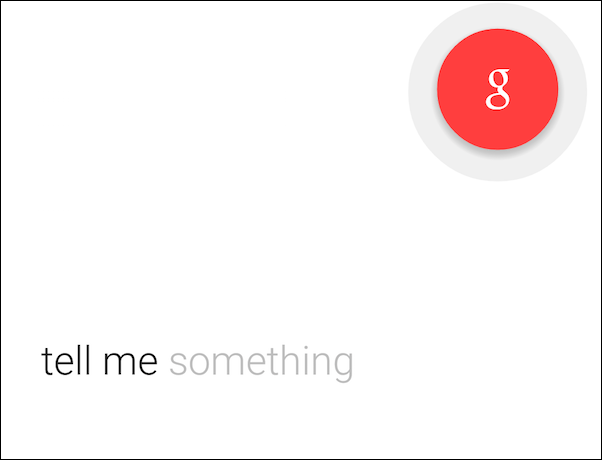
\includegraphics[width=10cm]{Pics/Chap2/google-voice.png}
  \caption{Giao diện chung của Google Voice Search}
\end{figure}

Một đặc điểm quan trọng cần kể đến của Google Speech Recognition API chính là khả năng trả về kết quả thời gian thực, tức là kết quả được trả về với từng từ mà người dùng vừa nhập vào và chưa kết thúc câu nói của mình. Tính năng này giúp cho việc phát triển các ứng dụng trở nên dễ dàng và linh hoạt hơn, không cần đợi đến khi người dùng kết thúc nói mới trả về kết quả. Tính năng này cũng chính là một phần quan trọng giúp cho đồ án định hướng được những giải pháp hữu ích cho vấn đề cần giải quyết.

Tuy nhiên, sự sai sót trong việc nhận diện là không thể tránh khỏi do những nguyên nhân như môi trường xung quanh quá ồn dẫn đến âm lượng giọng nói của người dùng chưa đủ lớn, hay tốc độ nói của người dùng quá nhanh dẫn đến những nhập nhằng trong âm thanh. Vì vậy, trong đồ án đã nghiên cứu tìm ra phương pháp hạn chế lại những sai sót đó để có thể nắm bắt tốt nhất yêu cầu từ phía người dùng, đó là sử dụng một mô hình ngôn ngữ (Language Model) sẽ được giới thiệu chi tiết hơn ở phần sau của đồ án.

\section{Xây dựng chatbot}
\subsection{Một vài nền tảng hỗ trợ xây dựng chatbot}

Chatbot như đã nêu ở trên là một phần mềm cho phép tạo ra những cuộc hội thoại mà người dùng có cảm giác như đang được nói chuyện với một người thật. Những chatbot đơn giản sử dụng công thức chung là pattern-matching, so sánh những dữ liệu đầu vào với một tập các câu nói có sẵn trong tập dữ liệu học và chọn ra câu trả lời phù hợp nhất. Tuy nhiên điều này không giúp ích nhiều cho những ứng dụng muốn thực hiện được những yêu cầu từ phía người dùng hay quan tâm đến những cách diễn đạt khác từ phía người dùng khi cùng đề cập đến một vấn đề, vì thực tế rằng những chatbot này chưa hiểu được yêu cầu từ phía người dùng. Để giải quyết vấn đề này, nhiều hệ thống đã tích hợp thêm khả năng về xử lý ngôn ngữ tự nhiên. Tuy nhiên việc xây dựng một hệ thống xử lý ngôn ngữ tự nhiên của riêng mình là điều mà các nền tảng hỗ trợ chatbot chưa làm được, vì vậy họ sử dụng những dịch vụ của 

\subsection{Vài nét về Wit.ai}

% \begin{table}[h]
% 	\caption{So sánh các phiên bản của Unity, theo trang chủ \textit{unity.com}}
% 	\centering
% 	\begin{tabular}{ | c | C | C | C | C | }
% 	\hline
% 	License & Cloud Build & Report hiệu năng & Loại bỏ Splash Screen & Quyền truy cập mã nguồn của Unity \\
% 	\hline
% 	Personal & Standard & Không & Không & Không \\
% 	\hline
% 	Plus & Priority & Có & Có & Không \\
% 	\hline
% 	Pro & Concurrent Builds & Có & Có & Không \\
% 	\hline
% 	Enterprise & Dedicated Build Agents & Có & Có & Có \\
% 	\hline
% 	\end{tabular}
% \end{table}


\section{Công cụ hỗ trợ quá trình phát triển}
Để quá trình phát triển diễn ra một cách trơn tru, dự án \project có sử dụng những công cụ hỗ trợ bên cạnh game engine và các công cụ sản xuất như Photoshop, 3DS Max và Maya. Những công cụ hỗ trợ này trải dài qua các khía cạnh khác nhau của dự án, giúp cho việc hợp tác giữa các thành viên tham gia trở nên dễ dàng.
\begin{itemize}
	\item \textbf{Dropbox}: Dùng để chia sẻ tài liệu và tài nguyên đồ họa giữa các thành viên với nhau. Công cụ này giúp cho các artist và designer luôn có bản cập nhật mới nhất của các tài nguyên sử dụng trong dự án một cách tự động.
	\item \textbf{Git}: Nếu như các artist và designer có dropbox thì lập trình viên sử dụng git để có thể thoải mái hợp tác với nhau hay tách ra làm một chức năng riêng biệt.
	\item \textbf{Trello}: Đóng vai trò như một trang liệt kê công việc và theo dõi bug.
\end{itemize}

\stopcontents[parts]

\part{Các kết quả đạt được}
\startcontents[parts]
\printcontents[parts]{}{-1}{\setcounter{tocdepth}{1}}
\chapter{Tổng quan}
\section{Mô tả kịch bản trò chơi}
Game \project, như đã nói ở trên, là một game bắn súng góc nhìn thứ nhất (FPS) trên mobile mà trong đó người chơi là một phi hành gia lạc vào một hành tinh khác và bị những quái vật trên hành tinh đó tấn công. Nhiệm vụ của người chơi là tiêu diệt hết những quái vật này và sống sót để qua màn chơi. Những quái vật này được chia làm ba cấp độ:
\begin{itemize}
	\item Quái thường - \textit{Basic}: Kích thước nhỏ, thường có tốc độ di chuyển khá nhanh và đi theo nhóm số lượng lớn, được chia làm hai nhóm nhỏ:
	\begin{itemize}
		\item Quái tấn công: Chúng sẽ tấn công người chơi với cường độ cao khi chúng đến đủ gần.
		\item Quái tự sát: Tốc độ di chuyển rất cao, khi đến chỗ người chơi chúng sẽ phát nổ và gây một lượng sát thương tương đối lớn.
	\end{itemize}
	\item Quái lớn - \textit{Elite}: Kích thước lớn, tuy di chuyển chậm và có cường độ tấn công thấp nhưng lượng sát thương lớn.
	\item Trùm - \textit{Boss}: Kích thước rất lớn, có những skills đặc biệt và đa dạng nhằm gây khó dễ cho người chơi khi tiêu diệt chúng.
\end{itemize}

Để hoàn thành màn chơi, người chơi sẽ được cung cấp các loại súng, vốn được thiết kế đa dạng (súng tiểu liên, súng máy, súng phóng tên lửa, súng phóng đạn đuổi, súng phóng lựu\ldots) nhằm phục vụ các phong cách chơi khác nhau. Bên cạnh các loại súng, người chơi có thể mang theo một số vật phẩm hỗ trợ như vật phẩm hồi máu, áo giáp hoặc tăng sát thương cho súng. Hệ thống súng và vật phẩm được gọi là tài sản (inventory). Người chơi hoàn toàn có thể mua thêm, nâng cấp hoặc thay thế các loại tài sản trên.

Ngoài các màn chơi chính, người chơi có thể chơi hai chế độ đặc biệt: phó bản (treasure) và vô hạn (endless). Chế độ phó bản cung cấp một số cơ chế đặc biệt như tốc độ nhanh hoặc tính giờ, trong khi đó ở chế độ vô hạn người chơi sẽ phải cố gắng sống sót càng lâu càng tốt trước những đợt quái ra liên tiếp. Hai chế độ đặc biệt này sẽ thêm màu sắc và sự đa dạng cho trò chơi.
\section{Các yêu cầu về chức năng}
\begin{itemize}
	\item Hệ thống quái vật: hành vi của từng con quái, AI.
	\item Hệ thống sinh quái theo thời gian hoặc theo đợt.
	\item Hệ thống súng và vật phẩm.
	\item Dữ liệu về tiến trình chơi của người dùng: các màn đã mở khóa, thông tin về chế độ phó bản và chế độ vô hạn cũng như tài sản hiện tại của người chơi.
\end{itemize}

\section{Các yêu cầu phi chức năng}
\begin{itemize}
	\item Game chạy trên nền tảng Android ($\geqslant$ 4.0)
	\item Game chạy ổn định với tối thiểu 30 khung hình trên một giây.
	\item Phong cách đồ họa low poly, dễ thương.
\end{itemize}

\chapter{Phân tích và thiết kế}
\section{Data-driven design}
\subsection{Data-driven design là gì?}
Data-driven design, trong phát triển game, là một tư tưởng nhằm đưa những giá trị hoặc hành vi của các thành phần trong game vào dữ liệu lưu trên đĩa cứng, thay vì được định nghĩa trong mã nguồn. Một ví dụ đơn giản của việc áp dụng data-driven design trong phát triển game đó là file lưu trữ những thiết lập của người chơi (player preferences). Các thông tin như âm lượng, độ phân giải màn hình hay thiết lập phím được lưu vào đây.

\subsection{Tại sao lại dùng data-driven design?}
Theo quan điểm của người viết, bất cứ game nào được xuất ra thị trường cũng có mục tiêu lớn nhất là đem lại một cảm xúc nhất định cho người chơi. Cảm xúc đó có thể khác nhau giữa các tựa game: cảm giác kinh hoàng với các tựa game kinh dị như \textit{Outlast}, cuồng nhiệt với \textit{Guitar Hero} hay buồn chán tột độ với \textit{Life Is Strange}. Xác định cảm xúc mà game sẽ truyền tải là yếu tố then chốt để định nghĩa giá trị cốt lõi của game. Tuy vậy, sau khi cảm xúc này được xác định, việc đảm bảo nó là không hề dễ dàng. Không ai có thể định nghĩa hay tiên đoán được cảm xúc mà một tính năng, một hiệu ứng trong game mang lại, cho đến khi thử nó. Do vậy, việc phát triển game yêu cầu thử đi thử lại liên tục, cho đến khi sản phẩm truyền tải được cảm xúc mà nó hướng tới.

Vào những ngày mà ngành công nghiệp phát triển game vẫn còn non trẻ, tất cả mọi thứ đều được lập trình trực tiếp (\textit{hardcoded}). Cái vợt trong trò chơi \textit{Pong} được tạo ra bằng một mảng một chiều chứa tọa độ các điểm làm nên cây vợt, để máy tính có thể biết được nên tô màu trắng nên những phần nào của màn hình. Giả sử khi người ta cần thay đổi độ dài của cái vợt, các bước phải thực hiện sẽ là: 1/ Chỉnh sửa kích thước và giá trị của mảng một chiều chứa tọa độ ở trên, 2/ Biên dịch (compile) lại chương trình và 3/ Chạy thử. Quy trình này được lặp đi lặp lại cho đến khi những người phát triển thấy hài lòng về độ dài của cái vợt. Nếu những thành phần khác cần được tinh chỉnh, quy trình dài dòng và mệt mỏi này lại được lặp lại, dù có thể thứ cần thay đổi chỉ là tăng một số nguyên lên 1 đơn vị.

Do bản chất yêu cầu việc thử đi thử lại liên tục, việc áp dụng quy trình trên gây ra rất nhiều lãng phí. Do đó các thông tin thay đổi liên tục, ví dụ như thông số của các thành phần trong game, hoặc những thay đổi mà người chơi tạo ra được đưa vào dữ liệu trên đĩa cứng. Việc này đem lại một vài lợi ích rõ ràng:
\begin{itemize}
	\item Game designer có thể thoải mái tinh chỉnh, cân bằng các thông số thay vì phải nhờ đến các lập trình viên, qua đó lập trình viên có thể tập trung vào làm việc với hệ thống hoặc lập trình các tính năng, mà không cần phải bận tâm đến việc tinh chỉnh thông số (thực ra, đó vốn là công việc của các game designer).
	\item Sau khi các thông số được tinh chỉnh, các game designer có thể thử nghiệm ngay lập tức mà không hề tốn thời gian chờ biên dịch lại, do các thông số này nằm hoàn toàn trên các file dữ liệu. Điều này đồng nghĩa với việc họ có thể tiến tới cảm xúc mà sản phẩm muốn truyền tải nhanh hơn.
\end{itemize}
\subsection{Áp dụng data-driven design trong \project}
Unity vốn là một data-driven game engine. Thực tế các đối tượng trong Unity được \textit{serialize}\footnote{Serialization: Quá trình lưu một đối tượng logic vào một định dạng có thể lưu được trên đĩa cứng hoặc truyền tải qua mạng.} vào các file dữ liệu. Cửa sổ Inspector đóng vai trò như một công cụ để xem và chỉnh sửa giá trị của các trường dữ liệu này. Khi viết các C\# script cho các đối tượng trong game, Unity sẽ \textit{serialize} các trường dữ liệu \texttt{public} hoặc có tag \texttt{[SerializeField]}. Như vậy, những yếu tố cần cân chỉnh liên tục như thời gian chạy hiệu ứng hoặc chỉ số của vật phẩm có thể được áp dụng kỹ thuật này, nhằm giảm thời gian phát triển và cho phép thử nghiệm liên tục.

Không chỉ hỗ trợ \textit{serialize} các đối tượng vào định dạng riêng của mình để theo dõi trên Inspector, Unity còn hỗ trợ \textit{serialize} vào các định dạng dữ liệu phổ biến như XML, JSON hoặc CSV. Như vậy, những dữ liệu mang tính hệ thống có thể được \textit{serialize} sang các định dạng phổ biến này, ví dụ như:
\begin{itemize}
	\item Dùng CSV cho thông tin sinh quái trong một màn chơi, vốn được tổ chức dạng bảng và có thể chỉnh sửa dễ dàng và trực quan trên Microsoft Excel
\begin{table}[h]
	\caption{Ví dụ về thông tin sinh quái trong một màn chơi (giản lược)}
	\centering
	\begin{tabular}{ | c | C | C | C | C | }
	\hline
	Wave & Spawn Time (s) & Enemy ID & Number & Spawn at gate \\
	\hline
	1 & 1 & 103 & 4 & 0 \\
	\hline
	1 & 2.5 & 103 & 5 & 2 \\
	\hline
	2 & 1 & 201 & 2 & 1 \\
	\hline
	3 & 1 & 202 & 1 & 3 \\
	\hline
	\end{tabular}
	\label{tab:enemywaves}
\end{table}
	\item Dùng JSON cho những thông tin về hệ thống súng, chỉ số của quái vật,\ldots để có thể chỉnh sửa nhanh bằng text editor mà không cần mở Unity editor.
\end{itemize}

\subsection{Kết luận}
Data-driven giúp tiết kiệm rất nhiều thời gian phát triển game, đặc biệt là trong giai đoạn tinh chỉnh những chi tiết nhỏ, khi mà những chỉ số như sát thương của quái hay tốc độ ra đạn của súng được chỉnh từng đơn vị nhỏ nhất. Các game designer có thể thử nghiệm ý tưởng của họ ngay lập tức mà không cần qua các bước trung gian như đồng bộ dữ liệu hoặc đợi bản build test, trong khi đó các lập trình viên sẽ không cần phải liên tục mở các file mã nguồn để sửa từng con số và mất thời gian chờ đợi các file này được dịch, thay vào đó họ có thể tập trung vào sửa các lỗi nghiêm trọng hoặc phát triển các tính năng mới.

Điểm bất lợi của data-driven đó là công đoạn chuẩn bị lâu hơn so với việc gán thẳng giá trị vào mã nguồn. Lập trình viên sẽ phải suy nghĩ nhiều hơn về hệ thống, thảo luận nhiều hơn với các game designer về các đặc điểm chung giữa các thực thể để thống nhất được những thông số cần cân chỉnh cũng như cách khớp chúng vào hệ thống hiện tại. Điều này không thực sự phù hợp trong giai đoạn thử nghiệm (prototype) hoặc đề xuất tính năng. Ngoài ra, các game designer, đặc biệt là những người không có nền tảng về lập trình, có thể vô tình gây ra lỗi khi thao tác trực tiếp với dữ liệu bằng cách nhập vào các giá trị không phù hợp.

\section{Kiến trúc dựa trên thành phần (component based)}
Trong lập trình hướng đối tượng, kế thừa (inheritance) là một kỹ thuật phổ biến cho việc tái sử dụng mã nguồn. Ý tưởng cơ bản của kế thừa là tổ chức các lớp đối tượng vào một cây (hierarchy), trong đó các lớp con sẽ sử dụng các thuộc tính và hành vi của lớp cha, và định nghĩa các hành vi riêng của chúng. Tuy nhiên, gần đây việc sử dụng quan hệ kế thừa đã thể hiện nhiều khuyết điểm, do đó nó bị thay thế bằng kiến trúc dựa trên thành phần, vốn đề cao việc sử dụng quan hệ kết tập (composition) hơn là kế thừa.
\subsection{Bất lợi của quan hệ kế thừa}
Đầu tiên, kế thừa sẽ làm tăng độ phức tạp của mã nguồn, bởi thuộc tính và hành vi của các lớp con phụ thuộc vào lớp cha. Mỗi thay đổi ở lớp cha sẽ ảnh hưởng trực tiếp tới tất cả các lớp con của lớp đó, cũng như các lớp kế thừa từ các lớp con này. Cây kế thừa càng sâu, sự ảnh hưởng này càng lớn và có khả năng gây lỗi cao hơn. Thêm vào đó, mỗi khi thêm một lớp vào cây kế thừa, lập trình viên sẽ phải nắm rõ các hoạt động của tất cả các lớp cơ sở của lớp này.\cite{codecomplete}

Như vậy, khi có một lỗi xảy ra, và lỗi nằm ở một lớp cha, lập trình viên sẽ phải tiến hành sửa lỗi trên lớp cha đó, và duyệt qua một lượt các lớp con để đảm bảo rằng sự thay đổi này không làm ảnh hưởng tới hoạt động của chúng. Tuy nhiên trường hợp xảy ra thường xuyên lại là có ảnh hưởng. Khi ấy, rất nhiều công sức phải bỏ ra để sửa các vấn đề này, dẫn tới giảm sút về tốc độ phát triển của toàn bộ dự án.

Ngoài ra, với những hệ thống đơn giản (giả sử hệ thống quái với ba con quái khác nhau), hệ thống dựa trên kế thừa có thể được triển khai mà không mất quá nhiều công thức. Tuy nhiên, khi hệ thống này được mở rộng, cây kế thừa cũ tỏ ra không quá linh hoạt, và một vài ``ngoại lệ'' được thêm vào, kèm theo đó là việc các lớp con ở tầng dưới của cây kế thừa sẽ chứa nhiều thuộc tính và hành vi thừa thãi. Với nhiều sự mở rộng hơn, cuối cùng kết quả thu được sẽ là một cây kế thừa phức tạp, trong khi đó lại hoàn toàn phi lý về mặt logic.
\begin{figure}[H]
  \centering
    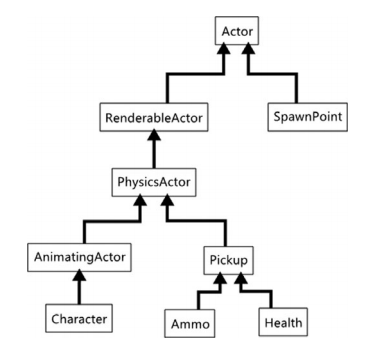
\includegraphics[width=10cm]{Pics/Chap4/inheritance.png}
  \caption{Một ví dụ về cây kế thừa phức tạp\cite{gamecodingcomplete}.} 
  \label{fig:hierarchy}
\end{figure}

Hình \ref{fig:hierarchy} mô tả một cây kế thừa phức tạp. Xuất phát từ lớp cơ sở \texttt{Actor}, lớp \texttt{RenderableActor} được tạo để làm lớp cơ sở cho \texttt{PhysicsActor}. Các nhân vật có thể được diễn hoạt (animate), nên lớp \texttt{Character} kế thừa từ \texttt{AnimatingActor}, vốn là một \texttt{PhysicsActor}. Khi nhu cầu cần thêm một đối tượng có thể được diễn hoạt nhưng lại không cần thiết phải chịu sự điều khiển của engine vật lý, ví dụ như một cái cây mang mục đích trang trí, thiết kế này sẽ nảy sinh vấn đề. Cách giải quyết thứ nhất là cho lớp \texttt{DecoratingTree} kế thừa từ \texttt{AnimatingActor}, như vậy lớp đó sẽ chứa những tính năng mà nó hoàn toàn không nên có. 

\begin{figure}[H]
  \centering
    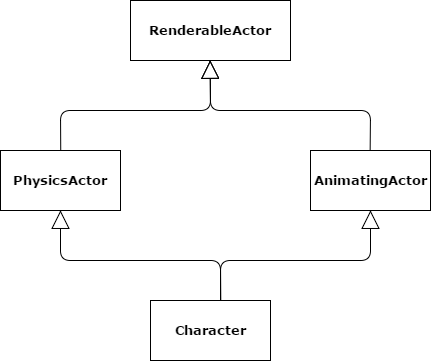
\includegraphics[width=7cm]{Pics/Chap4/multipleinheritance.png}
  \caption{Diamond of death.} 
  \label{fig:multipleinheritance}
\end{figure}
Cách giải quyết thứ hai là viết lại lớp \texttt{AnimatingActor} sao cho nó không còn kế thừa từ \texttt{PhysicsActor nữa}, nhưng như vậy thì \texttt{Character} sẽ phải kế thừa từ hai lớp cha. Đa kế thừa có rất nhiều vấn đề, đặc biệt trong số đó có vấn đề \textit{diamond of death}\footnote{Diamond of death: Hiện tượng một lớp có hai lớp cơ sở, nhưng hai lớp cơ sở này lại cùng kế thừa từ một lớp cơ sở khác. Điều này không chỉ gây ra mập mờ về việc đọc hiểu mã nguồn cho lập trình viên, nó có thể gây ra lỗi ngữ nghĩa liên quan tới những hàm ảo bị trùng lặp của các lớp cơ sở.} như trong hình \ref{fig:multipleinheritance}, và quan trọng nhất là ngôn ngữ C\# mà Unity sử dụng làm scripting language không hỗ trợ đa kế thừa.

Do những bất lợi kể trên, quan hệ kế thừa không phù hợp khi được dùng trong quá trình phát triển game, vốn có rất nhiều sự thay đổi không được báo trước. Những tính năng thừa thãi mà các lớp con phải mang theo cũng là một vấn đề cần giải quyết nhằm đảm bảo tính trong sáng và dễ bảo trì của mã nguồn.

\subsection{Chi tiết về kiến trúc hướng thành phần}
Kiến trúc hướng thành phần, như đã nói ở trên, sử dụng mối quan hệ kết tập thay vì lạm dụng quan hệ kế thừa. Tư tưởng chung của kiến trúc này là tách biệt các phần chức năng thành các thành phần (component) độc lập với nhau. Các thực thể trong game sẽ bao gồm một số lượng các thành phần này và có thể có bao gồm đoạn code quy định cách hoạt động của thực thể đó.
\begin{figure}[h]
  \centering
    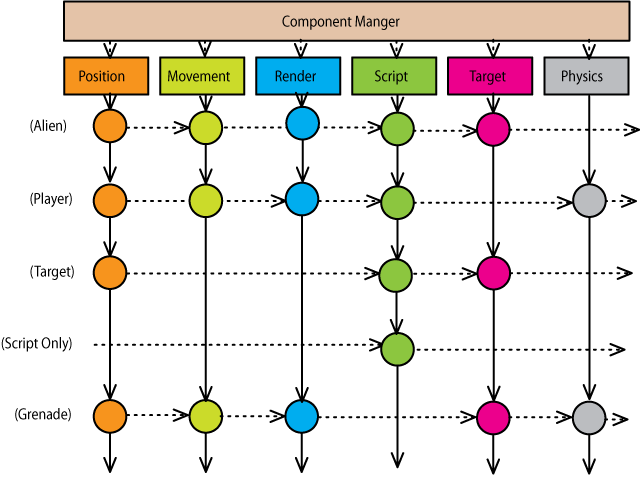
\includegraphics[width=14cm]{Pics/Chap4/components.png}
  \caption{Kiến trúc hướng thành phần.}
\end{figure}

\textit{Unreal Engine} sử dụng một hệ thống lai giữa hai kiến trúc kế thừa và thành phần. Tất cả các thực thể trong game sẽ là các \texttt{Actor}. Các \texttt{Actor} có thể được điều khiển bởi người chơi hoặc hệ thống AI được gọi là \texttt{Pawn}. Khi thêm vào các chức năng liên quan đến hành vi di chuyển của nhân vật, thành phần phát hiện va chạm và một mesh có xương (\texttt{SkeletalMeshComponent}) vào lớp \texttt{Pawn}, ta có lớp \texttt{Character}. \textit{Unreal Engine} vốn được phát triển dành cho dòng game FPS, nên các thực thể \texttt{Character} có thể chạy, đi bộ, bay và bơi trong thế giới game. Tất cả các \texttt{Actor} đều có thể được mở rộng tính năng bằng việc viết code trực tiếp kế thừa từ một trong ba lớp cơ sở thích hợp kể trên, hoặc gắn thêm cho nó một \texttt{ActorComponent}.

Trong khi đó, \textit{Unity} sử dụng cách tiếp cận dựa hoàn toàn trên kiến trúc thành phần. Một \texttt{GameObject} (tương tự khái niệm \texttt{Actor} trong \textit{Unreal Engine}, dùng để diễn tả một thực thể được đặt vào trong thế giới game) chỉ đơn thuần là một tập hợp các thành phần. Hành vi của nó hoàn toàn do các thành phần này quyết định. Khi viết một script \texttt{MonoBehavior} điều khiển \texttt{GameObject}, người dùng thực chất đang lập trình các hành vi của một component.

Cách tiếp cận này giúp người dùng có thể thoải mái lắp ghép để tạo nên một thực thể mong muốn. Muốn thực thể đó có thể hiện lên trong thế giới game? Gắn cho nó một \texttt{MeshRenderer}. Muốn nhân vật có thể diễn hoạt được? Gắn cho nó một \texttt{SkeletalMeshRenderer} và một \texttt{Animator}. Muốn thực thể đó chịu tác động của vật lý? Gắn cho nó một \texttt{Rigidbody}. Khi yêu cầu thay đổi và một trong những tính năng kể trên không còn cần thiết nữa? Chỉ cần loại bỏ những thành phần liên quan là xong.

Kiến trúc này đảm bảo sự tách biệt tốt giữa các thành phần với nhau, đồng nghĩa với việc các tính năng có thể phát triển hoặc thay đổi độc lập mà không quá lo lắng với việc gây ảnh hưởng tới những phần còn lại. Ví dụ, thành phần vật lý có thể không cần biết tới sự tồn tại của thành phần hiển thị, hoặc thành phần diễn hoạt không quan tâm tới thành phần tìm đường. Tuy nhiên có những trường hợp không lý tưởng, thành phần này vẫn cần phải biết tới sự tồn tại của thành phần kia, như trường hợp của thành phần diễn hoạt và thành phần hiển thị, hay thành phần tìm đường và vị trí. Trong trường hợp này, việc đảm bảo liên lạc hiệu quả giữa các thành phần với nhau là cần thiết. Có ba phương án có thể cân nhắc tới\cite{gameprogrammingpatterns}:
\begin{itemize}
	\item Chỉnh sửa trực tiếp trạng thái của thực thể:
	\begin{itemize}
		\item Các thành phần được giữ tách biệt khỏi nhau.
		\item Thứ tự thực hiện thay đổi tại thực thể là quan trọng.
	\end{itemize}
	\item Tham chiếu trực tiếp tới thành phần khác:
	\begin{itemize}
		\item Đơn giản.
		\item Gây ra sự phụ thuộc giữa hai thành phần.
	\end{itemize}
	\item Gửi thông điệp hoặc phát sự kiện:
	\begin{itemize}
		\item Tương đối phức tạp để thực hiện.
		\item Đảm bảo tính tách biệt.
	\end{itemize}
\end{itemize}

Cách đầu tiên, chỉnh sửa trực tiếp trạng thái của thực thể không thể thực hiện được trong \textit{Unity} do đặc thù kỹ thuật của engine. Hai cách còn lại, cách nào cũng có những điểm mạnh và điểm yếu riêng, do đó cả hai đều được sử dụng trong việc áp dụng kiến trúc dựa trên thành phần vào dự án, điều này sẽ được trình bày trong tiểu mục tiếp theo. Cần chú ý rằng, kiến trúc hướng thành phần không hề loại bỏ hoàn toàn quan hệ kế thừa, quan hệ này vẫn được sử dụng trong những trường hợp mà nó phát huy tác dụng như cần thống nhất về kiểu dữ liệu hoặc tận dụng lợi thế của các hảm ảo.

\subsection{Áp dụng kiến trúc hướng thành phần vào \project}
Do Unity vốn sử dụng hệ thống dựa trên thành phần, nên những script được thêm vào các thực thể của game đã là những component. Tuy nhiên, có những thành phần đặc biệt được thiết kế để dùng đi dùng lại giữa nhiều thực thể với nhau, hoặc được tổ chức một cách có hệ thống. Tiểu mục này sẽ trình bày những hệ thống component quan trọng, cũng như các chúng giao tiếp với nhau.

\subsubsection{Hệ thống quái}
Theo thiết kế sơ bộ, các con quái sẽ có những thành phần sau:
\begin{itemize}
	\item \texttt{BaseEnemy}: Ngoài việc lưu trữ các thông tin liên quan tới quái (được load từ file config), lớp \texttt{BaseEnemy} lưu giữ một danh sách các \texttt{EnemyController} điều khiển hành vi của quái cũng như cách truy cập tới những \texttt{EnemyController} này.
	\item \texttt{EnemyController}: Cung cấp các hành vi chung của các thành phần điều khiển enemy, cũng như các hàm khởi tạo giá trị hoặc dọn dẹp dùng trong pattern tối ưu hiệu năng Object Pool (mục \ref{sec:pool}).
	\item Các thành phần \texttt{EnemyController} liên quan tới các công việc đặc thù như animation, di chuyển, tấn công cũng như hệ thống ra quyết định\footnote{Xem mục \ref{sec:decisiontree}}.
\end{itemize}

Ngoài ra, quái vật có thể có những thành phần phụ trợ mà không phải là các \texttt{EnemyController}, do chúng không cần phải được khởi tạo lại giá trị với pattern Object Pooling, ví dụ như:
\begin{itemize}
	\item Thành phần điều khiển hiệu ứng quái chìm xuống dưới lòng đất sau khi nó bị giết.
	\item Thành phần vẽ đường đạn cho các loại quái có súng.
	\item Thành phần điều khiển những loại hiệu ứng đặc biệt của một vài loại quái (ví dụ quái hệ Elite có hiệu ứng đất bắn lên khi chạy).
\end{itemize}

Mối quan hệ giữa các thành phần được mô tả trong hình \ref{fig:enemyclasses}.

\begin{figure}[H]
  \centering
    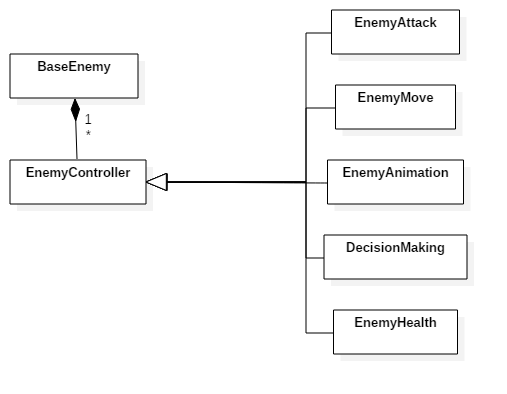
\includegraphics[width=13cm]{Pics/Chap4/Enemy.png}
  \caption{Thiết kế lớp sơ bộ cho hệ thống quái.}
  \label{fig:enemyclasses}
\end{figure}

Hầu hết các thành phần này sử dụng phương pháp tham chiếu trực tiếp để truy cập tới một thành phần khác bất kỳ, trừ một vài trường hợp đặc thù mà phương pháp phát sự kiện tỏ ra hiệu quả hơn:
\begin{itemize}
	\item Sự kiện tấn công: animation tấn công của quái được gọi trực tiếp từ trong mã nguồn, tuy nhiên việc người chơi mất máu trước khi đòn tấn công của quái tiếp cận là bất hợp lý. Sự kiện tấn công sẽ được phát khi animation tấn công này chạy tới một khung hình đặc biệt, khi đó người chơi mới bị mất máu.
	\item Sự kiện kết thúc animation chết: với những quái vật không thuộc dòng tự sát, sau khi chết nó sẽ chìm xuống dưới đất. Khi ấy, sự kiện kết thúc animation chết của quái sẽ được phát ra.
\end{itemize}

Unity hỗ trợ thiết lập các hàm callback liên quan đến các sự kiện được phát ra ngay trên cửa sổ Inspector, vì thế việc thiết lập các sự kiện này khá trực quan và đơn giản, cũng như đảm bảo tính dùng lại của các thành phần. Bất lợi duy nhất của nó là khi có lỗi xảy ra, việc truy tìm các lời gọi hàm là tương đối phức tạp vì các lời gọi hàm này được lưu trữ trong các file dữ liệu và được load lên lúc run-time.

\subsubsection{Hệ thống súng và đạn}
Tương tự với hệ thống quái, hệ thống súng và đạn cũng được xây dựng trên cơ sở gồm Base và danh sách các Controller, với súng là \texttt{BaseGun} và \texttt{GunController} còn với đạn là \texttt{BaseBullet} và \texttt{BulletController}. Các lớp Base giữ các thông tin cơ bản của đối tượng, trong khi đó các lớp Controller được dùng để thống nhất về kiểu dữ liệu hoặc cung cấp một khung hành vi chung giữa các thực thể khác nhau.
\begin{figure}[H]
  \centering
    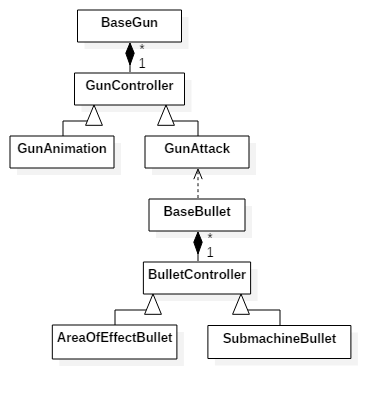
\includegraphics[width=10cm]{Pics/Chap4/Gun.png}
  \caption{Thiết kế lớp sơ bộ cho hệ thống súng và đạn.}
  \label{fig:gunclasses}
\end{figure}

Để tránh trùng lặp dữ liệu, thông tin của \texttt{BaseGun} được đọc từ file config lưu trên đĩa cứng theo cách làm tương tự với quái, nhưng thông tin của \texttt{BaseBullet} (mức độ sát thương, thời gian sống...) sẽ được quyết định khi viên đạn được sinh ra dựa vào thông tin của \texttt{BaseGun} cung cấp. Như vậy, khi cần thay đổi sát thương của một khẩu súng, các game designer không cần phải chỉnh sửa cùng một thông tin ở hai chỗ, ngoài ra việc thay đổi trực tiếp tại thông tin của súng giúp họ có thể tính toán cân bằng các thông số tốt hơn.

\subsubsection{Các thành phần hỗ trợ khác}
Bên cạnh các thành phần đặc thù như trên, một vài thành phần hỗ trợ cũng được thêm vào nhằm phục vụ nhiều mục đích. Những thành phần hỗ trợ quan trọng bao gồm:
\begin{itemize}
	\item \texttt{CameraFacingBillboard}: Đảm bảo các đối tượng được gắn thành phần này luôn nhìn về hướng của camera. Thanh máu của quái, hiệu ứng critical shoot\footnote{Hiệu ứng dùng sát thương lớn đột ngột so với sát thương thông thường. Trong \project, hiệu ứng này để tạo cảm giác mạnh mẽ cho người chơi.} hoặc các cây giả 3D được gắn thành phần này.
	\item \texttt{AutoRecycle}: Với các đối tượng có thời gian sống hữu hạn, việc gắn thành phần này vào sẽ đảm bảo các đối tượng này chỉ hoạt động trong thời gian sống của nó. Hết thời gian sống, nó sẽ được ``cất'' vào một chỗ để dùng lại trong tương lai (sẽ được trình bày chi tiết hơn trong mục \ref{sec:pool}. Object Pooling)
	\item \texttt{GravitySimulator}: Có những đối tượng mà việc nó rơi xuống nhanh hơn tác động của trọng lực sẽ tạo cảm giác tốt hơn, ví dụ như viên đạn của súng phóng lựu hoặc quả bom mà một loại quái Elite ném vào người chơi. Thành phần này đơn giản là nhân tác động của trọng lực lên đối tượng với một hệ số để tạo hiệu ứng đối tượng rơi nhanh hay chậm.
	\item \texttt{AudioClipsList}: Unity có sẵn thành phần \texttt{AudioSource} phục vụ việc chơi âm thanh (cả nhạc nền và hiệu ứng). Tuy nhiên có những đối tượng cần nhiều hơn một hiệu ứng âm thanh như súng (âm thanh đổi súng, âm thanh bắn\ldots) hay quái (âm thanh tấn công, âm thanh bị mất máu, âm thanh bị giết,\ldots). Thành phần này lưu một dãy các cặp <tên hiệu ứng> - <file âm thanh> để tiện cho việc chơi các hiệu ứng khi cần.
\end{itemize}

\section{Thiết kế giao diện và luồng hoạt động của game}
\subsection{Luồng hoạt động của game}
\subsection{Thiết kế giao diện}

\chapter{Các vấn đề kỹ thuật}
\section{Các cơ chế đáng chú ý trong game}

\subsection{Cơ chế bắn súng}
Quá trình bắn súng được chia làm hai công đoạn chính. Công đoạn thứ nhất liên quan tới việc tạo ra viên đạn, thiết lập hướng bay cùng vận tốc ban đầu cho nó. Sau đó, viên đạn sẽ được khởi tạo các thông số logic như sát thương, tầm sát thương hoặc thời gian sống. Công đoạn thứ hai chỉ thuần túy là gán các giá trị đọc được từ dữ liệu của khẩu súng, vì vậy mục này sẽ tập trung giải thích cách tính toán đường bay của viên đạn.

Đầu tiên, để có được hướng bay của viên đạn, hai điểm biểu thị điểm xuất phát và điểm đích của nó phải được xác định. Với điểm xuất phát, bản thân dữ liệu về khung xương của model của khẩu súng đã có một xương (joint) biểu diễn đầu súng, tọa độ hiện tại của xương này trong hệ tọa độ chung (world space) sẽ là điểm xuất phát của viên đạn.

Với điểm đích, cần tìm được vị trí người chơi đang ngắm đến trong hệ tọa độ chung. Dựa vào vị trí hiện tại và hướng nhìn của người chơi, ta tạo một tia\footnote{Tia (\textit{Ray}): là một đường thẳng có điểm xuất phát và hướng trong một hệ tọa độ bất kỳ. Độ dài của tia là hữu hạn trong hệ tọa độ đó.} có độ dài bằng khoảng bắn xa nhất của người chơi. Tuy nhiên, không phải lúc nào người chơi cũng có chủ đích ngắm bắn tại điểm xa nhất có thể. Với trường hợp có đối tượng cần bắn đứng gần, cơ chế kể trên có thể bị sai lệch (xem hình \ref{fig:shootingwrong}).

\begin{figure}[H]
  \centering
    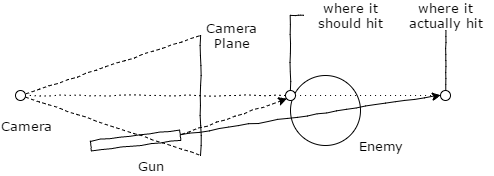
\includegraphics[width=10cm]{Pics/Chap5/shootingwrong.png}
  \caption{Trường hợp gây sai lệch cảm giác bắn.}
  \label{fig:shootingwrong}
\end{figure}

Như vậy, nếu tia ở trên có chiếu qua một vật có thể bắn được (địa hình, cây cối, đá hoặc quái\ldots) thì điểm đích sẽ là vị trí va chạm gần nhất của tia với vật đó. Unity cung cấp cơ chế tính điểm này bằng khái niệm \textit{Raycast}.

Cơ chế này hoạt động tốt với các loại súng phóng lựu hoặc súng phóng tên lửa, bởi chúng có tốc độ ra đạn thấp. Với các loại súng máy, do tốc độ ra đạn nhanh, cần phải giảm xác suất trúng đích xuống dưới 100\% bằng độ giật của súng. Để đạt được điều này, thay vì bắn vào vị trí ngắm được xác định, đích đến $T$ của viên đạn sẽ được làm nhiễu theo công thức:
\[
T = t + n
\]
với $t$ là đích ngắm, $n$ là độ nhiễu, là một vector 3 chiều với các trường $x$, $y$, $z$ được lấy ngẫu nhiên trong khoảng $(-noise, noise)$. Độ giật $noise$ sẽ tăng dần đến cực đại khi người chơi giữ nút bắn, và giảm dần khi người chơi nhả nút bắn ra.

\begin{figure}[h]
  \centering
    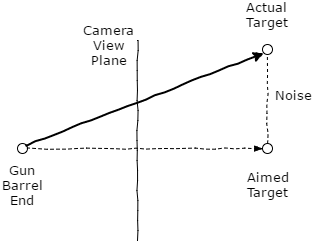
\includegraphics[width=10cm]{Pics/Chap5/shootingmechanic.png}
  \caption{Minh họa cơ chế bắn súng có độ nhiễu.}
\end{figure}

\subsection{Cảnh báo quái đang đến bằng mũi tên}
Vì trò chơi mang tính casual nhẹ nhàng, việc cần phải quay liên tục để xem xung quanh mình có gì sẽ khiến người chơi cảm thấy khó khăn và mệt mỏi. Thêm vào đó, do đặc thù của dòng game FPS trên mobile, việc quay liên tục mang lại trải nghiệm khó khăn hơn so với việc dùng chuột trên PC. Vì vậy, những mũi tên cảnh báo sẽ trở nên có ích.

Mũi tên cảnh báo sẽ chỉ cho người chơi thấy có quái vật đang tiến đến mà người chơi không nhìn thấy, còn với những quái vật mà người chơi đang quan sát thì việc có mũi tên chỉ hướng không những không giúp ích gì mà còn có thể gây phân tâm.
\begin{figure}[H]
  \centering
    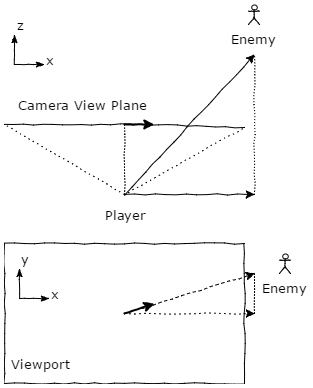
\includegraphics[width=9cm]{Pics/Chap5/indicator.png}
  \caption{Minh họa cách tính toán hướng của mũi tên cảnh báo (nhìn theo mặt phẳng $xz$ và $xy$ trong hệ tọa độ cục bộ của người chơi).}
\end{figure}

Góc quay của mũi tên cảnh báo sẽ được tính theo công thức:
\[ \alpha = \arccos (projection.y) \]
với $projection$ là kết quả phép chiếu vector hướng từ người chơi đến quái vật lên mặt phẳng $xy$ trong hệ tọa độ cục bộ của người chơi. Kết quả thu được như sau:
\begin{figure}[H]
  \centering
    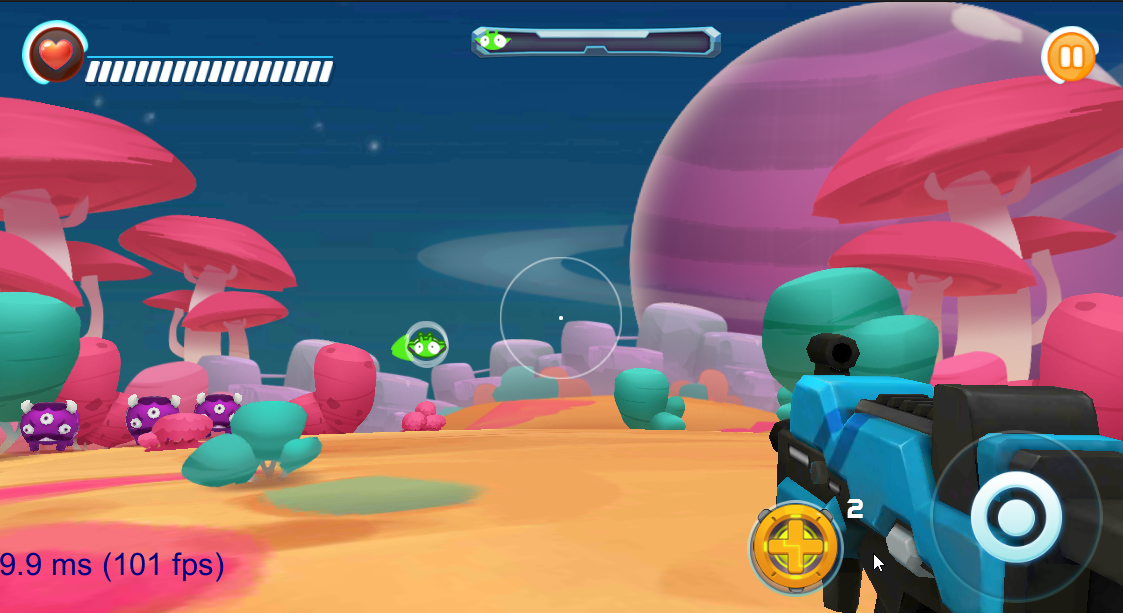
\includegraphics[width=14cm]{Pics/Chap5/indicatordemo.png}
  \caption{Mũi tên chỉ hướng sau khi được đưa vào game.}
\end{figure}

Việc kiểm tra quái vật có nằm trong vùng nhìn thấy của người chơi hay không được thực hiện nhờ vào vùng quan sát của camera\footnote{Camera view frustum: Là vùng mà một camera có thể quan sát được, có hình dạng là hình chóp tứ giác cụt.}. Các \textit{Mesh} của quái vật, nếu thỏa mãn điều kiện AABB\footnote{Axially Aligned Bounding Box: hình hộp bao quanh model 3D, được xác định bởi hai điểm góc $p_{min} = [x_{min}, y_{min}, z_{min}]$ và $p_{max} = [x_{max}, y_{max}, z_{max}]$} của chúng nằm một phần trong hình chóp cụt quan sát của camera, sẽ được tính là nhìn thấy. Ngược lại, quái vật này sẽ nằm ngoài vùng nhìn, và nó sẽ phải được đưa vào danh sách cảnh báo bằng mũi tên.
\begin{figure}[H]
  \centering
    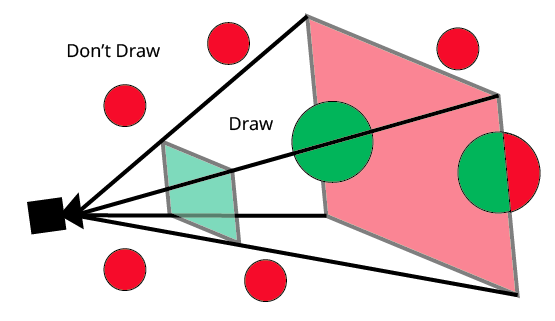
\includegraphics[width=8cm]{Pics/Chap5/camerafrustum.png}
  \caption{Vùng quan sát của camera.}
\end{figure}

\section{Cây quyết định}
\label{sec:decisiontree}
Cây quyết định (\textit{decision tree}) là một kỹ thuật rất phổ biến trong phát triển các thành phần AI, không chỉ trong game mà còn trong các hệ thống thương mai. Điểm mạnh của cây quyết định là nhanh, dễ cài đặt và dễ hiểu\cite{aiforgames}. Mục này sẽ trình bày sơ qua về các nguyên tắc chung của cây quyết định và cách nó được áp dụng vào \project.

\subsection{Sơ bộ về cây quyết định}
Một cây quyết định được tạo thành bởi nhiều nút, mỗi nút tương ứng với một điểm quyết định. Khi ra quyết định, tác tử sẽ bắt đầu cân nhắc các khả năng từ nút gốc của cây quyết định cho tới khi nó tới được một nút lá, tương ứng với một hành động.

\begin{figure}[h]
  \centering
    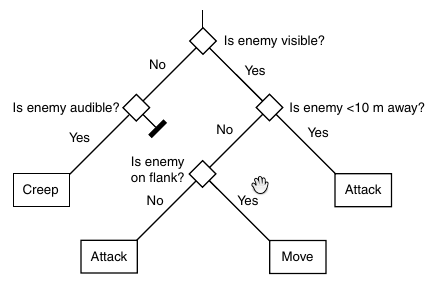
\includegraphics[width=10cm]{Pics/Chap5/dectree.png}
  \caption{Ví dụ một cây quyết định\cite{aiforgames}.}
  \label{fig:dectreeexample}
\end{figure}

Hình \ref{fig:dectreeexample} cho thấy ví dụ về một cây quyết định đơn giản. Các nút hình thoi được gọi là nút quyết định (decision node). Điều kiện gắn với nút quyết định sẽ trả về kết quả đúng hoặc sai, nhờ vậy mà tác tử có thể xác định được đường đi trên cây quyết định. Các nút hành động (action node) được biểu diễn bằng các hình chữ nhật. Khi quá trình ra quyết định của tác tử chạm tới một nút lá, hành động gắn với nó sẽ được thực hiện ngay lập tức. Cần chú ý là các nút con của nút quyết định không cần thiết phải là một nút hành động, vì rõ ràng có những trường hợp chúng ta có nhiều điều kiện cần cân nhắc.

\begin{figure}[h]
  \centering
    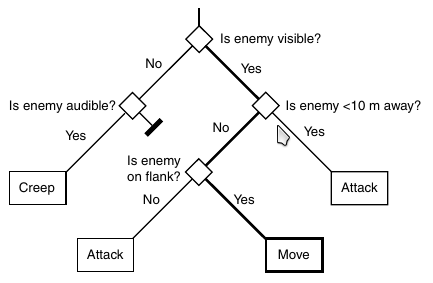
\includegraphics[width=10cm]{Pics/Chap5/dectreetravelled.png}
  \caption{Ví dụ quá trình ra quyết định.}
  \label{fig:dectree2example}
\end{figure}

Hình \ref{fig:dectree2example} cho thấy quá trình một tác tử ra quyết định bằng đường màu đậm, dựa trên những gì nó quan sát được.

Thuật toán cây quyết định có độ phức tạp là $O(n \log _2 n)$, với $n$ là số nút quyết định trên cây cùng giả định thời gian thực hiện các nút quyết định hoặc hành động là $O(1)$. Tuy nhiên thực tế thì có khá nhiều điều kiện hoặc hành động tốn nhiều thời gian hơn $O(1)$, ví dụ như để kiểm tra xem có kẻ địch ở gần mình hay không, tác tử phải duyệt qua danh sách kẻ địch và tính khoảng cách từ bản thân tới chúng. Hành động này sẽ có độ phức tạp là $O(n_{enemy})$.

\subsection{Thực hiện}
Với các cấu trúc dữ liệu đệ quy\footnote{Một cấu trúc dữ liệu A được gọi là \textit{đệ quy} khi nó chứa giá trị cũng có kiểu dữ liệu A trong định nghĩa của nó. Các cấu trúc dữ liệu thông dụng có thể được cài đặt một cách đệ quy là danh sách liên kết hoặc cây.}, giải thuật đệ quy là giải pháp phù hợp bởi tính dễ hiểu, dễ cài đặt của nó. Bộ nhớ cho các lời gọi hàm đệ quy được cấp phát trong bộ nhớ \textit{stack}, do đó tốc độ cấp phát là rất nhanh do cơ chế LIFO (last in first out), tuy nhiên bộ nhớ này có thể bị đầy nhanh chóng\footnote{Gây ra hiện tượng \textit{stack overflow}}.

\begin{lstlisting}[frame=lines, basicstyle=\footnotesize\ttfamily, numbers=left, numberstyle=\tiny\color{black},caption= {Interface \texttt{IDecisionTreeNode}}, backgroundcolor=\color{background}]
public interface IDecisionTreeNode
{
	float MakeDecision();
}
\end{lstlisting}

Các cấu trúc dữ liệu biểu diễn các nút trên cây kế thừa từ interface \texttt{IDecisionTreeNode}. Interface này cung cấp hàm \texttt{MakeDecision} để thực hiện việc ra quyết định. Đầu tiên là lớp \texttt{DecisionNode}. Lớp này chứa tham chiếu đến hai nút tiếp theo, tương ứng với giá trị trả về của điều kiện \texttt{condition()} là đúng hay sai.

\begin{lstlisting}[frame=lines, basicstyle=\footnotesize\ttfamily, numbers=left, numberstyle=\tiny\color{black},caption= {Lớp \texttt{DecisionNode}}, backgroundcolor=\color{background}]
public delegate bool DecisionFunction();

public class DecisionNode : IDecisionTreeNode
{
	private IDecisionTreeNode trueNode;
	private IDecisionTreeNode falseNode;
	DecisionFunction condition;

	public float MakeDecision()
	{
		if (condition())
		{
			return trueNode.MakeDecision();
		}
		else
		{
			return falseNode.MakeDecision();
		}
	}
}
\end{lstlisting}

Lớp \texttt{ActionNode} chứa một hàm \texttt{action} tượng trưng cho hành động đi kèm với nút. Cần chú ý rằng, giá trị trả về của hàm \texttt{MakeDecision} là một số thực. Giá trị này biểu diễn \textit{thời gian cần thiết} để thực hiện hành động.

Tác tử sẽ nghĩ \textit{sau khi} hành động gần nhất được thực hiện. Điều này đảm bảo tính linh hoạt cho cây quyết định, ví dụ như tác tử có thể di chuyển và dừng lại ngay lập tức để tấn công, hoặc khi nó đang tấn công thì nó sẽ không ``nghĩ'' cho đến khi nó thực hiện xong đợt tấn công đó.

\begin{lstlisting}[frame=lines, basicstyle=\footnotesize\ttfamily, numbers=left, numberstyle=\tiny\color{black},caption= {Lớp \texttt{ActionNode}}, backgroundcolor=\color{background}]
public delegate void ActionFunction();

public class ActionNode : IDecisionTreeNode
{
	ActionFunction action;
	float actionDuration;

	public float MakeDecision()
	{
		if (action != null)
		{
			action();

			return actionDuration;
		}

		return 0;
	}
}
\end{lstlisting}

Bên cạnh hai loại nút trên, thực tế chỉ ra cho thấy có những trường hợp tác tử cần thực hiện một \textit{chuỗi hành động liên tiếp}. Ví dụ, khi đến gần vị trí của người chơi, kẻ địch sẽ phải dừng lại và quan sát xem có được đánh không (giả sử, nó vừa tấn công người chơi và phải chờ đến hết lượt nghỉ mới được đánh tiếp). Do vậy lớp \texttt{SequenceNode} được tạo ra nhằm phục vụ mục đích đó. Mỗi nút tuần tự chứa một danh sách các nút cần phải thực hiện tiếp theo. Các nút này có thể là nút quyết định, nút hành động hoặc nút tuần tự.

\begin{lstlisting}[frame=lines, basicstyle=\footnotesize\ttfamily, numbers=left, numberstyle=\tiny\color{black},caption= {Lớp \texttt{SequenceNode}}, backgroundcolor=\color{background}]
public class SequenceNode : IDecisionTreeNode
{
	private IDecisionTreeNode[] nodesToPerform;

	public float MakeDecision()
	{
		float actionDuration = 0;
		for (int i = 0; i < nodesToPerform.Length; i++)
		{
			actionDuration += nodesToPerform[i].MakeDecision();
		}

		return actionDuration;
	}
}
\end{lstlisting}

Với sự xuất hiện của nút tuần tự, cây quyết định có thể được viết với sự linh hoạt lớn hơn. Hình \ref{fig:dectreereal} minh hoạ một cây quyết định với nút tuần tự (nút hình tam giác). Thực tế, đây chính là một trong những cây quyết định được sử dụng trong dự án \project.
\begin{figure}[H]
  \centering
    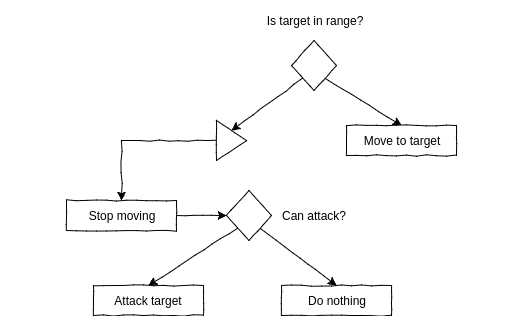
\includegraphics[width=13cm]{Pics/Chap5/realdectree.png}
  \caption{Ví dụ cây quyết định với nút tuần tự.}
  \label{fig:dectreereal}
\end{figure}

Để tái sử dụng mã nguồn, mỗi NPC\footnote{Non playable character: các nhân vật do máy điều khiển.} sẽ được trang bị một \textit{component} phục vụ việc ra quyết định. Luồng hoạt động của component này như sau:
\begin{enumerate}
	\item Đọc dữ liệu về cây quyết định được sử dụng của NPC.
	\item Xây dựng cây dữ liệu và trả về một nút gốc \texttt{IDecisionTreeNode}.
	\item Mỗi lần nghĩ sẽ duyệt cây quyết định một lần để đưa ra quyết định phù hợp.
\end{enumerate}

Để biểu diễn dữ liệu của cây quyết định, JSON là một lựa chọn phù hợp vì nó đơn giản, dễ đọc hiểu với những người không phải lập trình viên, và phổ biến. Ngoài ra, JSON có thể được hình ảnh hoá thành một biểu đồ dạng cây, giúp cho các game designer có thể hình dung ra luồng hoạt động của NPC trong thực tế. 
\begin{lstlisting}[frame=lines, language=json, basicstyle=\footnotesize\ttfamily, numbers=left, numberstyle=\tiny\color{black},caption= {Một file JSON mô tả cây quyết định}]
{
  "type": "decision",
  "condition": "isTargetInRange",
  "trueNode": {
    "type": "sequence",
    "nodesToPerform": [
      {
        "type": "action",
        "action": "stop"
      },
      {
        "type": "decision",
        "condition": "canAttack",
        "trueNode": {
          "type": "action",
          "action": "attackTarget"
        },
        "falseNode": {
          "type": "action",
          "action": "doNothing"
        }
      }
    ]
  },
  "falseNode": {
    "type": "action",
    "action": "moveToTarget"
  }
}
\end{lstlisting}

\section{Tối ưu}
Khác với các sản phẩm khác, bất chấp việc phần cứng ngày càng nhanh và mạnh mẽ, game vẫn yêu cầu phải vắt kiệt từng vòng lặp của CPU hay tận dụng từng byte bộ nhớ. 

\subsection{Object Pooling}
\label{sec:pool}
Kỹ thuật tối ưu đầu tiên là Object Pooling. 

\subsection{AutomaticLOD}
\label{sec:autolod}
\subsection{Custom shader: Unlit}

\chapter{Kết quả đạt được}
\chapter{Cài đặt và đánh giá}

\stopcontents[parts]

\chapter*{Kết luận}
\addtocontents{toc}{\bigskip}
\addcontentsline{toc}{chapter}{Kết luận}

\begin{thebibliography}{9}
\bibitem{aiforgames} 
Ian Millington and John Funge. 
\textit{Artificial Intelligence for Games}. 
Morgan Kaufmann Publishers, 2006.

\bibitem{codecomplete} 
Steve McConnell. 
\textit{Code Complete: A Practical Handbook of Software Construction, Second Edition}. 
Microsoft Press, 2004.

\bibitem{gameprogrammingpatterns} 
Robert Nystrom. 
\textit{Game Programming Patterns}. 
Genever Bennin, 2014.

\bibitem{gamecodingcomplete} 
Mike McShaffry and David "Rez" Graham. 
\textit{Game Coding Complete, Fourth Edition}. 
Cengage Learning, 2012.

\bibitem{3dmath} 
Fletcher Dunn., Ian Parberry
\textit{3D math primer for graphics and game development}. 
CRC Press, 2011.

\bibitem{unityorunrealformobile}
Sebastian Weber.
\textit{Unreal vs. Unity - Which engine is better for mobile games?}.
http://www.makinggames.biz/feature/unreal-vs-unity-which-engine-is-better-for-mobile-games,8472.html,
last visited March 2017.

\bibitem{datadriven}
Kyle Wilson.
\textit{Data-Driven Design}.
http://gamearchitect.net/Articles/DataDrivenDesign.html,
last visited March 2017.

\bibitem{componentbased}
Ray Wenderlich.
\textit{Introduction to Component Based Architecture in Games}.
https://www.raywenderlich.com/24878/introduction-to-component-based-architecture-in-games,
last visited November 2016.


\end{thebibliography}

\addcontentsline{toc}{chapter}{Tài liệu tham khảo}

\end{document}